\documentclass{article}
\usepackage{graphicx}
\usepackage[margin=1.5cm]{geometry}
\usepackage{amsmath}

\begin{document}

\title{Thursday Warm Up Exercise: Chapter 3-1 through 3-6}
\author{Prof. Jordan C. Hanson}

\maketitle

\section{Logic Gates: AND, OR, NOT}

\begin{enumerate}
\item Consider the circuit diagram in Fig. \ref{fig:plane}. Recall that the small circles represent NOT gates, before or after the AND and OR gates.  (a) If the left side of the landing gear is extended, but the right side of the landing gear is not, and the forward landing gear is extended, what will be the state of the LEDs? (b) If all three pieces of the landing gear are retracted, what will be the state of the LEDs? (c) If all three pieces of landing gear are extended, what will be the state of the LEDs? (d) Based on these observations, what does the green LED indicate? \\ \vspace{2.5cm}
\item Design a system that performs differently than the system in Fig. \ref{fig:plane}.  That is, the green LED is lit when all three pieces of landing gear are retracted, and the red LED is lit when any one piece of landing gear is extended. \\ \vspace{2.5cm}
\end{enumerate}

\section{Logic Gates: NAND, NOR, XOR, XNOR}

\begin{enumerate}
\item (a) Write the truth table (TT) for the AND gate, and then add a column for an AND gate followed by a NOT gate (NAND). (b) Write the TT for the NOR gate, an OR followed by a NOT. \\ \vspace{1cm}
\end{enumerate}

\begin{figure}[hb]
\centering
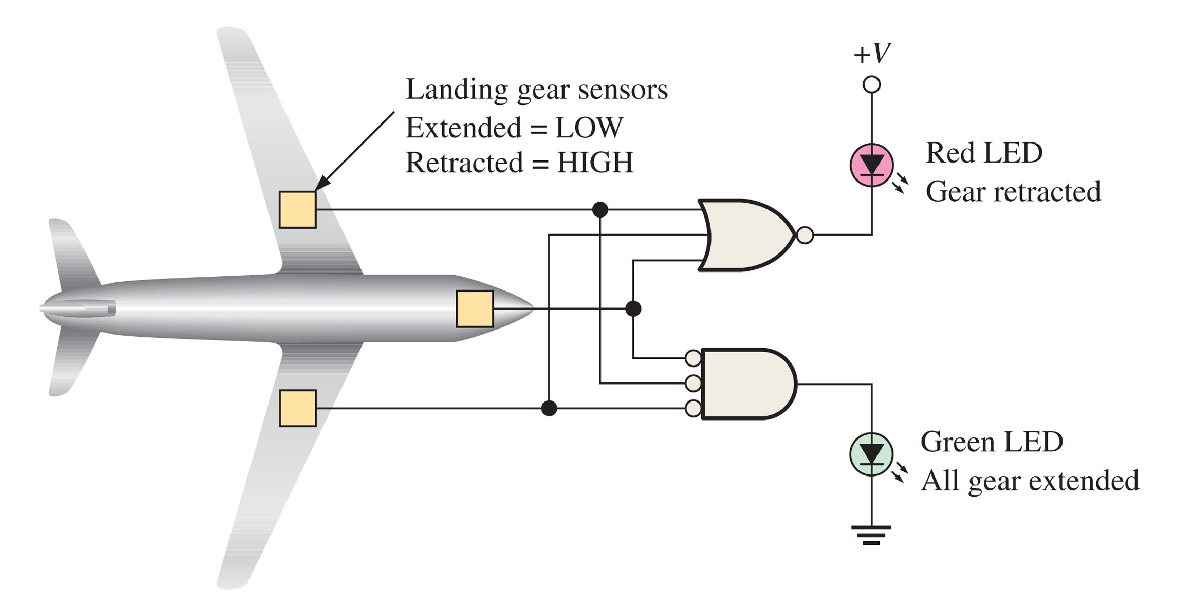
\includegraphics[width=0.5\textwidth]{figures/plane.pdf}
\caption{\label{fig:plane} A simple warning-light system for the landing gear of a passenger aircraft.}
\end{figure}

\end{document}
